\Aufgabe[10]{Tabellenbeziehungen}{
    \begin{enumerate}
        \item Visualisiere (mit Bleistift), wer Häuptling in welchem Dorf ist.
        \item Überlege, wie du allgemein für diese zwei Tabellen darstellen kannst, wie sie (und ihre Spalten) miteinander in Beziehung stehen.
    \end{enumerate}

    \centering
    \ifbeamer\vspace{-1cm}\fi
    \begin{tikzpicture}
        \node[inner sep=0pt] (imgdorf01) at (1,1) {%
             
\includegraphics[width=0.25\textwidth]{_Aufgaben/img/A05/A05_Dorf_01.png}
        };
        \node[inner sep=0pt, below=-1pt of imgdorf01] (imgdorf02) {%
             
\includegraphics[width=0.25\textwidth]{_Aufgaben/img/A05/A05_Dorf_02.png}
        };
        \node[inner sep=0pt, below=-1pt of imgdorf02] (imgdorf03)  {%
             
\includegraphics[width=0.25\textwidth]{_Aufgaben/img/A05/A05_Dorf_03.png}
        };
        \node[inner sep=0pt, below=-1pt of imgdorf03] (imgdorf04) {%
             
\includegraphics[width=0.25\textwidth]{_Aufgaben/img/A05/A05_Dorf_04.png}
        };
        \node[inner sep=0pt, below=-1pt of imgdorf04] (imgdorf05)  {%
             
\includegraphics[width=0.25\textwidth]{_Aufgaben/img/A05/A05_Dorf_05b.png}
        };
        
        \node[inner sep=0pt, right = 2cm of imgdorf01] (imgbew01) {%
             
\includegraphics[width=0.55\textwidth]{_Aufgaben/img/A05/A05_Bew_01.png}
        };
        \node[inner sep=0pt, below=-1pt of imgbew01] (imgbew02) {%
             
\includegraphics[width=0.55\textwidth]{_Aufgaben/img/A05/A05_Bew_02.png}
        };
        \node[inner sep=0pt, below=-1pt of imgbew02] (imgbew03) {%
             
\includegraphics[width=0.55\textwidth]{_Aufgaben/img/A05/A05_Bew_03.png}
        };
        \node[inner sep=0pt, below=-1pt of imgbew03] (imgbew04) {%
             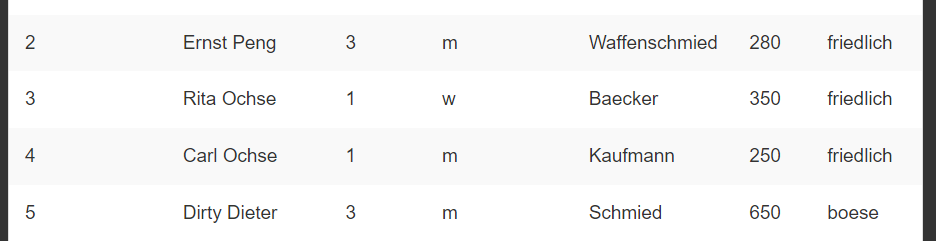
\includegraphics[width=0.55\textwidth]{_Aufgaben/img/A05/A05_Bew_04.png}
        };
        \node[inner sep=0pt, below=-1pt of imgbew04] (imgbew05) {%
             
\includegraphics[width=0.55\textwidth]{_Aufgaben/img/A05/A05_Bew_05.png}
        };
        \node[inner sep=0pt, below=-1pt of imgbew05] (imgbew06) {%
             
\includegraphics[width=0.55\textwidth]{_Aufgaben/img/A05/A05_Bew_06b.png}
        };
        \node[inner sep=0pt, below=-1pt of imgbew06] (imgbew07) {%
             
\includegraphics[width=0.55\textwidth]{_Aufgaben/img/A05/A05_Bew_07b.png}
        };
        %\Loesung{\draw[arrow] (imgdorf02) -- (imgbew02);}
        \Loesung{\draw[-{angle 60}, colA] (imgdorf03.east) to[out=0, in=180] (imgbew03.west);}
        \Loesung{\draw[-{angle 60}, colB] (imgdorf04.east) to[out=0, in=180] (imgbew05.west);}
        \Loesung{\draw[-{angle 60}, colC] (imgdorf05.east) to[out=0, in=180] (imgbew06.west);}
        \Loesung{\draw[-{angle 60}, red] (imgdorf02.north east) ++(-1cm, 0) to[out=45, in=180] (imgbew02.west) ;}
        \Loesung{\draw[-{angle 60}, red] (imgbew02.north) ++(-1cm, 0) to[out=150, in=25] ([shift={(-1.5cm, 0)}]imgdorf02.north);}

        %\node[above left = 0pt and 1pt of imgbew02, red] {1};
    \end{tikzpicture}
    
}

\UnterAufgabe[10]{Tabellenbeziehung im Klassendiagramm}{
    \ifbeamer\else\emphColB{Tabellenbeziehung im Klassendiagramm}\fi
    \begin{enumerate}
        \item Ergänze das Klassendiagramm entsprechend der beiden Tabellen oben.
        \item Wie kann man die Beziehungen zwischen den beiden Tabellen im Klassendiagramm darstellen?\\
            Tipp: Unsere Überlegungen von oben, helfen dabei.
    \end{enumerate}

{
    \ifloesung 
        %\color{\LFarbe}
        \renewcommand{\umldrawcolor}{\LFarbe}
        \renewcommand{\umltextcolor}{\LFarbe}
        \fontspec{Comic Sans MS} 
    \fi
    \begin{tikzpicture}
        \begin{class}[text width=7cm]{Dorf}{0,-1}
            \attribute{\ifloesung int dorfnr\fi}
            \attribute{\ifloesung String name\fi}
            \attribute{}
            \attribute{}
            \attribute{}
            \attribute{}
        \end{class}
        \begin{class}[text width=7cm]{Bewohner}{11,0}
            \attribute{\ifloesung int bewohnernr\fi}
            \attribute{\ifloesung String name\fi}
            \attribute{\ifloesung String geschlecht\fi}
            \attribute{\ifloesung String beruf\fi}
            \attribute{\ifloesung int gold\fi}
            \attribute{\ifloesung String status\fi}
            \attribute{}
            \attribute{}
            \attribute{}
            \attribute{}
            \attribute{}
        \end{class}
        \Loesung{\unidirectionalAssociation{Dorf}{1}{haeuptling}{Bewohner}}
    \end{tikzpicture}
    
    \renewcommand{\umldrawcolor}{\TFarbe}
    \renewcommand{\umltextcolor}{\TFarbe}
    }
}
